\begin{frame}{LLaVA: Visual Instruction Tuning}
  \begin{columns}[T,onlytextwidth]
    \column{0.50\textwidth}
      \begin{itemize}\footnotesize\itemsep0.35em
        \item \textbf{The gap.} Instruction tuning needs instruction-response pairs. Image-caption pairs were plentiful, image instructions with answers scarce, and crowd-sourcing them ``time-consuming and less well-defined''.
        \item \textbf{LLaVA} (Large Language and Vision Assistant; Liu et al., NeurIPS 2023), presented as the first attempt to extend instruction tuning to images, contributes:
        \begin{itemize}\scriptsize\itemsep0.1em
          \item \textbf{data:} 158K image instructions with answers, written by a text-only GPT-4;
          \item \textbf{a model:} CLIP encoder, one projection matrix, Vicuna; fine-tuned on ScienceQA (21K multiple-choice science questions) and ensembled with GPT-4, a new state of the art there: 92.53\%;
          \item \textbf{a benchmark:} LLaVA-Bench, scored by a GPT-4 judge;
          \item open data, code, checkpoints and demo.
        \end{itemize}
        \item This is the LLaVA-style recipe (covered earlier): frozen encoder, small projector, instruction tuning.
      \end{itemize}
    \column{0.48\textwidth}
      {\scriptsize\raggedright \textbf{Prompt} (an example from the GPT-4 report; the photo shows a man ironing clothes on a board fixed to the back of a yellow taxi): ``What is unusual about this image?''\par}
      \vspace{0.4em}
      \centering
      {\scriptsize\setlength{\tabcolsep}{4pt}
      \begin{tabular}{>{\raggedright\arraybackslash}p{1.7cm} >{\raggedright\arraybackslash}p{4.1cm}}
        \toprule
        \textbf{Model} & \textbf{Answer (verbatim)} \\
        \midrule
        BLIP-2 & a man is sitting on the back of a yellow cab \\
        \addlinespace[0.2em]
        OpenFlamingo & The man is drying his clothes on the hood of his car. \\
        \addlinespace[0.2em]
        LLaVA & The unusual aspect of this image is a man ironing clothes on the back of a minivan or van. This is not a typical place to perform this activity\ldots \\
        \bottomrule
      \end{tabular}\par}
      \vspace{0.4em}
      {\scriptsize\raggedright BLIP-2 and OpenFlamingo (both earlier in this lecture) describe the scene; LLaVA answers the question. Liu et al., ``Visual Instruction Tuning,'' NeurIPS 2023, \href{https://arxiv.org/abs/2304.08485v2}{arXiv:2304.08485v2}, Table~3.\par}
  \end{columns}
\end{frame}

\begin{frame}{Writing Image Instructions with a Text-Only LLM}
  \begin{columns}[T,onlytextwidth]
    \column{0.47\textwidth}
      \begin{itemize}\footnotesize\itemsep0.35em
        \item \textbf{Cheap baseline:} make the caption $\mathbf{X}_c$ of an image $\mathbf{X}_v$ the answer to a request $\mathbf{X}_q$ such as ``Describe the image concisely.'' It ``lacks diversity and in-depth reasoning''.
        \item \textbf{Symbolic image:} the teacher is language-only GPT-4, so each COCO image (covered earlier) is written out as text: its five captions and, for descriptions and reasoning, its object boxes (class name, four coordinates).
        \item \textbf{Prompt} (conversation type): ``You are an AI visual assistant, and you are seeing a single image.'' A few hand-written examples per type serve as in-context examples (covered earlier), the only human annotations in the pipeline.
        \item In early tests GPT-4 wrote better data than ChatGPT, for example on spatial reasoning.
      \end{itemize}
    \column{0.51\textwidth}
      \centering
      {\scriptsize\setlength{\tabcolsep}{4pt}
      \begin{tabular}{>{\raggedright\arraybackslash}p{1.65cm} >{\raggedright\arraybackslash}p{3.6cm} r}
        \toprule
        \textbf{Response type} & \textbf{What GPT-4 is asked to write} & \textbf{Samples} \\
        \midrule
        Conversation & multi-turn questions and answers on object types, counts, actions, locations and relative positions; only questions with definite answers & 58K \\
        \addlinespace[0.25em]
        Detailed description & a full description, requested by a question drawn at random from a fixed list & 23K \\
        \addlinespace[0.25em]
        Complex reasoning & questions whose answers need step-by-step reasoning about the scene & 77K \\
        \midrule
        \textbf{Total} & LLaVA-Instruct-158K, on 80K unique COCO images & \textbf{158K} \\
        \bottomrule
      \end{tabular}\par}
      \vspace{0.4em}
      {\scriptsize Liu et al., \href{https://arxiv.org/abs/2304.08485v2}{arXiv:2304.08485v2}, Sections~3 and~5.1; prompt from Table~13.\par}
  \end{columns}
\end{frame}

\begin{frame}{One COCO Image, Three Kinds of Instructions}
  \begin{columns}[T,onlytextwidth]
    \column{0.42\textwidth}
      \centering
      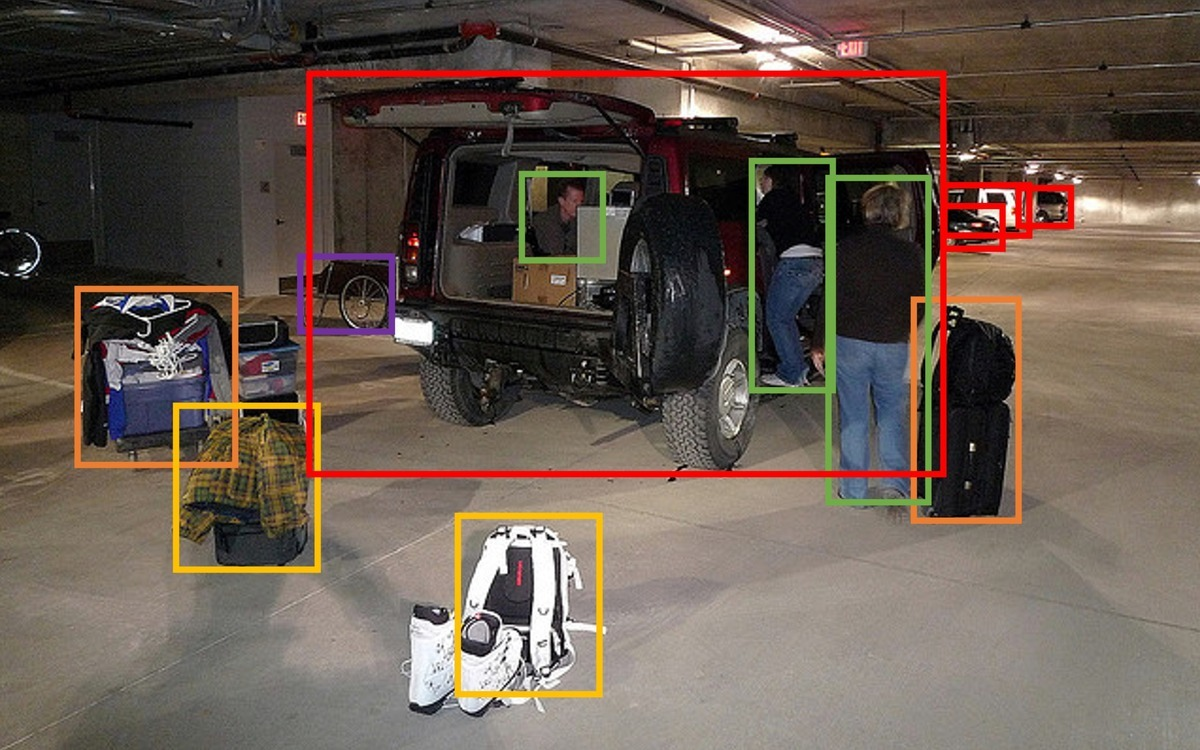
\includegraphics[width=\linewidth,height=0.30\textheight,keepaspectratio]{images/vision-language-models/llava_table1_coco_boxes.jpg}\\[0.2em]
      {\scriptsize Photo and text adapted from Liu et al., \href{https://arxiv.org/abs/2304.08485v2}{arXiv:2304.08485v2}, Table~1 (full text in Table~14; cuts marked \ldots). GPT-4 never saw the photo.\par}
      \vspace{0.5em}
      {\scriptsize\raggedright \textbf{What GPT-4 reads}\\[0.2em]
      \textbf{Captions} (2 of 5): A group of people standing outside of a black vehicle with various luggage. People try to fit all of their luggage in an SUV.\\[0.2em]
      \textbf{Boxes} (2 of 12; not given for conversations): person: [0.681, 0.242, 0.774, 0.694], backpack: [0.384, 0.696, 0.485, 0.914], \ldots\par}
    \column{0.56\textwidth}
      {\footnotesize\raggedright \textbf{What GPT-4 writes}\\[0.4em]
      \textbf{1. Conversation} (three turns; the first shown)\\
      Q: What type of vehicle is featured in the image?\\
      A: The image features a black sport utility vehicle (SUV).\\[0.5em]
      \textbf{2. Detailed description}\\
      The image is an underground parking area with a black sport utility vehicle (SUV) parked. There are three people in the scene, \ldots{} They are all working together to pack their luggage into the SUV for a trip. \ldots\\[0.5em]
      \textbf{3. Complex reasoning}\\
      Q: What challenges do these people face?\\
      A: \ldots{} They are facing the challenge of fitting all their luggage into the black SUV. There are multiple suitcases and backpacks to be packed, which suggests that the group has a significant amount of belongings \ldots\par}
  \end{columns}
  \vspace{0.3em}
  {\scriptsize GPT-4 writes as if it saw the photo; the authors later note these descriptions ``may contain a small amount of hallucinated content'' (Liu et al., ``Improved Baselines with Visual Instruction Tuning,'' CVPR 2024, \href{https://arxiv.org/abs/2310.03744v2}{arXiv:2310.03744v2}, Sec.~5.2).\par}
\end{frame}

\begin{frame}{LLaVA: Architecture}
  \begin{columns}[T,onlytextwidth]
    \column{0.52\textwidth}
      \centering
      \vspace{0.2em}
      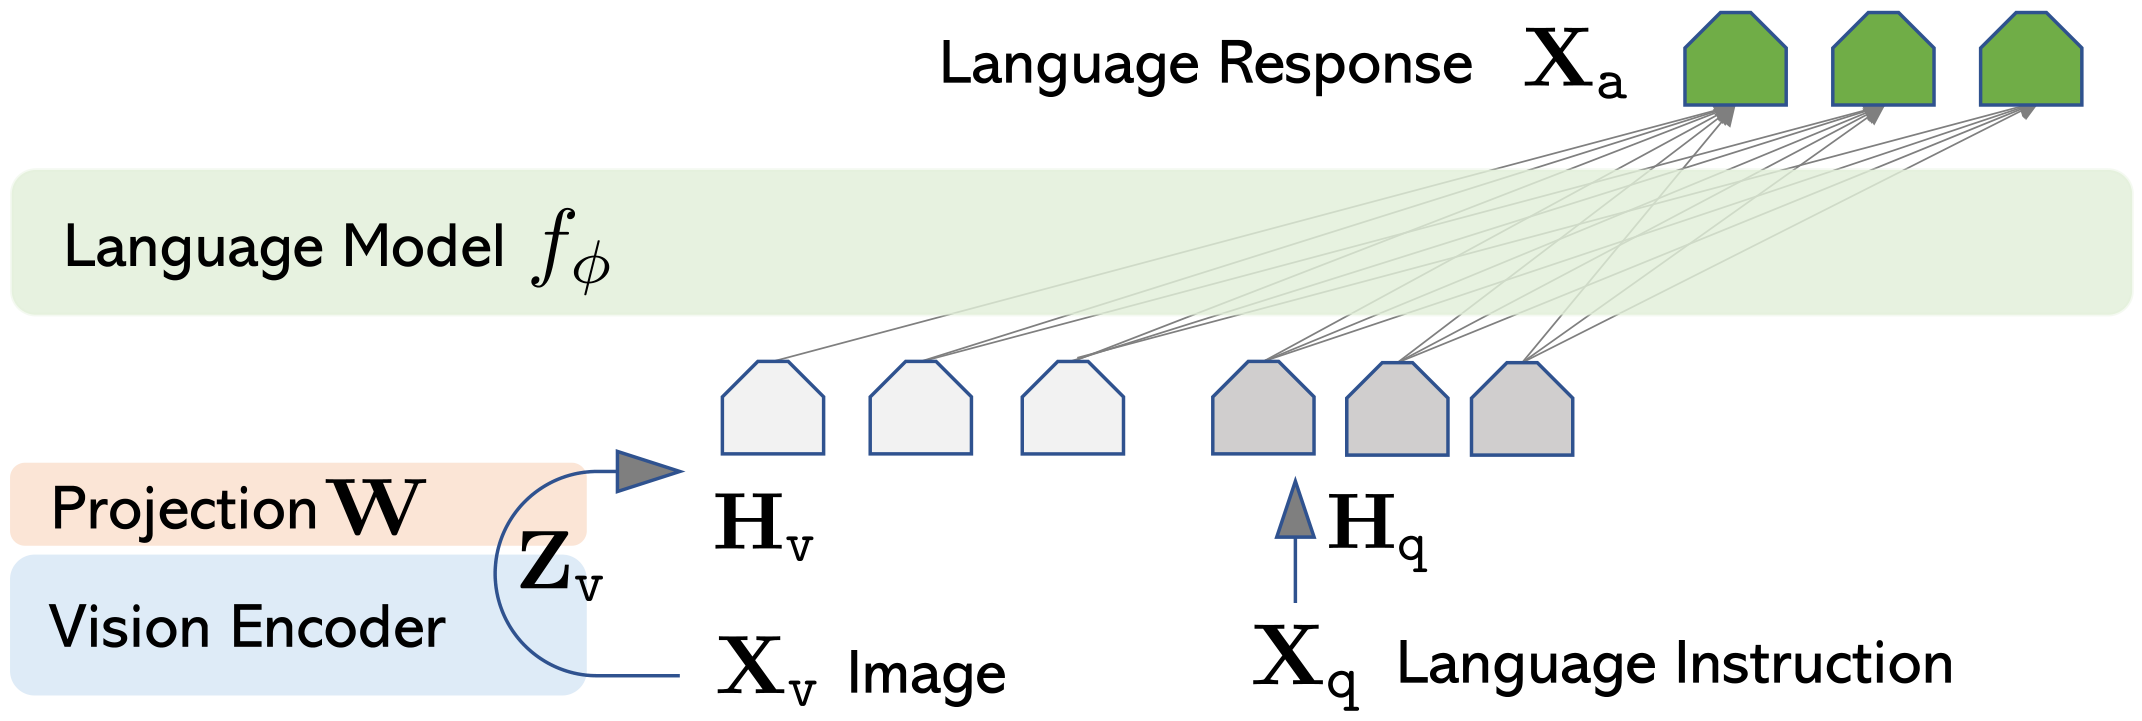
\includegraphics[width=\linewidth,height=0.40\textheight,keepaspectratio]{images/vision-language-models/llava_fig1_architecture.png}\\[0.2em]
      {\scriptsize Liu et al., \href{https://arxiv.org/abs/2304.08485v2}{arXiv:2304.08485v2}, Figure~1.\par}
      \vspace{0.3em}
      {\footnotesize
      \[ \mathbf{H}_v = \mathbf{W}\cdot\mathbf{Z}_v, \qquad \mathbf{Z}_v = g(\mathbf{X}_v) \]
      \raggedright $\mathbf{X}_v$: the image; $g$: the frozen CLIP image encoder; $\mathbf{Z}_v$: its grid of patch features; $\mathbf{W}$: a trainable projection matrix; $\mathbf{H}_v$: visual tokens as wide as the LLM's word embeddings; $\mathbf{H}_q$: the embedded instruction $\mathbf{X}_q$; $f_\phi$: the LLM (Vicuna) with weights $\phi$; $\mathbf{X}_a$: the answer.\par}
    \column{0.46\textwidth}
      \begin{itemize}\footnotesize\itemsep0.4em
        \item \textbf{Encoder:} CLIP ViT-L/14 (covered earlier), the Large ViT on $14\times14$-pixel patches. LLaVA reads the grid features from before its last layer; in an ablation they beat the last layer's, which the authors attribute to more local detail.
        \item \textbf{Projection:} one linear map, shared by all grid features, from 1,024 to 5,120 dimensions for the 13B LLM: about 5.2M weights.
        \item \textbf{Tokens:} a $224\times224$ image gives $(224/14)^2 = 16\times16 = 256$ visual tokens, placed before or after the first question.
        \item \textbf{Why so simple:} a light connector lets data experiments iterate fast; Flamingo's gated cross-attention and BLIP-2's Q-Former were left for future work.
      \end{itemize}
  \end{columns}
  \vspace{0.2em}
  {\scriptsize Widths and layer: released LLaVA-13B config, \href{https://huggingface.co/liuhaotian/LLaVA-13b-delta-v0/blob/main/config.json}{huggingface.co/liuhaotian/LLaVA-13b-delta-v0}. Layer ablation: Liu et al., \href{https://arxiv.org/abs/2304.08485v2}{arXiv:2304.08485v2}, Section~5.2 and Table~8.\par}
\end{frame}

\begin{frame}{Training: Align First, Then Instruct}
  \footnotesize
  Both stages maximize the likelihood of the assistant's answers:
  \[ p(\mathbf{X}_a \mid \mathbf{X}_v, \mathbf{X}_q) = \prod_{i=1}^{L} p_{\theta}\big(x_i \mid \mathbf{X}_v, \mathbf{X}_{q,<i}, \mathbf{X}_{a,<i}\big) \]
  $x_i$: the token being predicted; $\mathbf{X}_{q,<i}$, $\mathbf{X}_{a,<i}$: the instruction and answer tokens before it; $L$: sequence length; $\theta$: the trainable parameters. Only answer tokens and the \#\#\# stop marker carry loss.

  \vspace{0.2em}
  {\centering\scriptsize\setlength{\tabcolsep}{4pt}
  \begin{tabular}{>{\raggedright\arraybackslash}p{1.2cm} >{\raggedright\arraybackslash}p{6.0cm} >{\raggedright\arraybackslash}p{5.8cm}}
    \toprule
     & \textbf{Stage 1: feature alignment} & \textbf{Stage 2: end-to-end fine-tuning} \\
    \midrule
    Data & 595K CC3M pairs, balanced over concepts; the caption answers a brief-description request & LLaVA-Instruct-158K, the three response types sampled uniformly \\
    \addlinespace[0.15em]
    Trained & $\theta = \mathbf{W}$; CLIP and LLM frozen & $\theta = \{\mathbf{W}, \phi\}$; CLIP frozen \\
    \addlinespace[0.15em]
    Cost & 1 epoch, within 4 hours on 8 A100 GPUs & 3 epochs, within 10 hours on 8 A100 GPUs \\
    \bottomrule
  \end{tabular}\par}
  \vspace{0.2em}
  \begin{itemize}\itemsep0.25em
    \item \textbf{Stage 1} trains ``a compatible visual tokenizer for the frozen LLM''; in the variant fine-tuned on ScienceQA in stage 2, skipping it lowers accuracy from 90.92\% to 85.81\%.
    \item \textbf{Stage 2} lifts the LLaVA-Bench (COCO) relative score from 21.5\% to 85.1\%: a GPT-4 judge rates LLaVA's answers against those of a text-only GPT-4 that read the true captions and boxes.
  \end{itemize}
  \vspace{0.1em}
  {\scriptsize CC3M: Conceptual Captions, about 3.3M web images with cleaned alt-text captions (Sharma et al., ACL 2018, \href{https://aclanthology.org/P18-1238/}{aclanthology.org/P18-1238}). Liu et al., \href{https://arxiv.org/abs/2304.08485v2}{arXiv:2304.08485v2}, Secs.~4.2 and~5, App.~C, Tables~2, 4 and~8.\par}
\end{frame}

\begin{frame}{LLaVA-1.5: What Changed}
  \begin{columns}[T,onlytextwidth]
    \column{0.58\textwidth}
      \begin{itemize}\footnotesize\itemsep0.3em
        \item \textbf{Connector:} a two-layer MLP replaces the linear $\mathbf{W}$, the linear-to-MLP switch that helped SimCLR (covered earlier).
        \item \textbf{Encoder:} CLIP ViT-L/14 at 336 px, the highest resolution CLIP offers: $(336/14)^2 = 24\times24 = 576$ visual tokens.
        \item \textbf{Format prompt:} LLaVA ``tends to answer yes for yes/no questions'' and falls short on one-word-answer benchmarks. LLaVA-1.5 appends ``Answer the question using a single word or phrase.'' to short-answer visual question answering (VQA) data, so the answer format follows the prompt.
        \item \textbf{Data:} 558K BLIP-captioned pairs for alignment, then 665K instructions: LLaVA-Instruct-158K, 40K text-only ChatGPT conversations (ShareGPT), and eight VQA, region and OCR (text-reading) sets such as VQAv2 and RefCOCO (referring expressions: phrases that each pick out one object in a COCO image); about 1.2M public samples.
        \item \textbf{Cost:} about 6 hours of alignment and 20 hours of instruction tuning on one 8-A100 node, about a day for the 13B model; state of the art on 11 of its 12 benchmarks.
      \end{itemize}
    \column{0.40\textwidth}
      \centering
      \vspace{0.3em}
      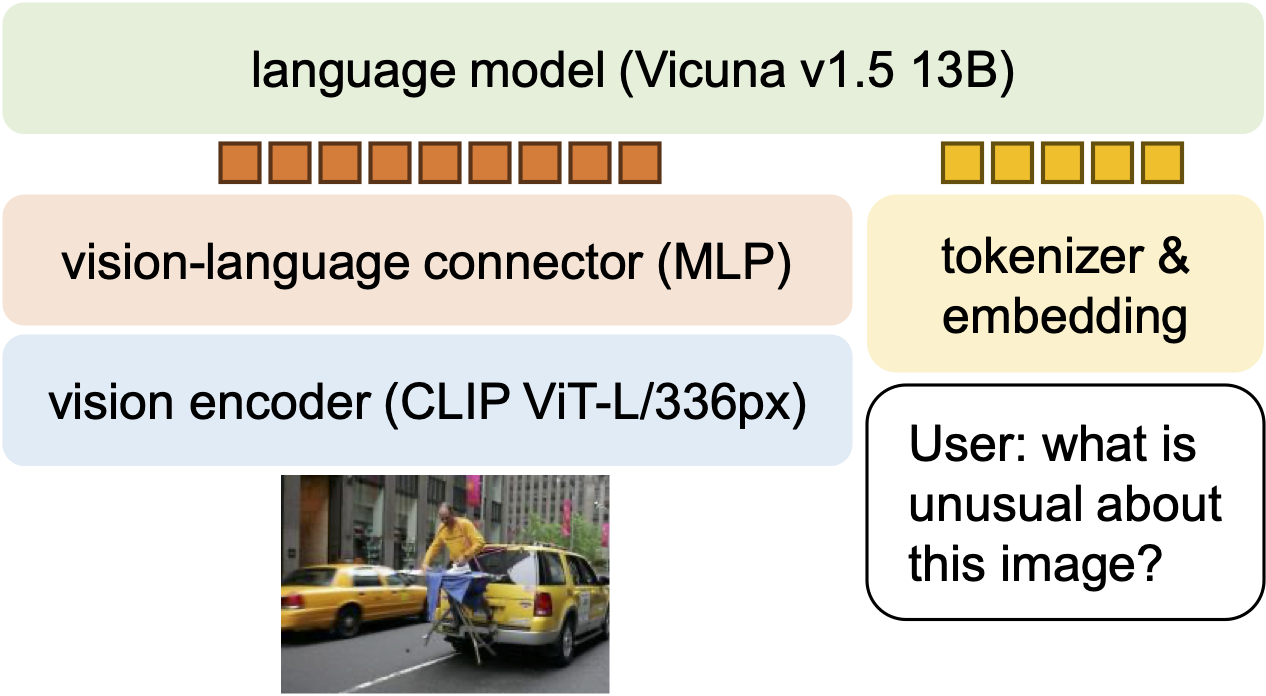
\includegraphics[width=\linewidth,height=0.46\textheight,keepaspectratio]{images/vision-language-models/llava15_fig1_mlp_connector.png}\\[0.2em]
      {\scriptsize Liu et al., \href{https://arxiv.org/abs/2310.03744v2}{arXiv:2310.03744v2}, Figure~1 (right panel); Sections~3.1--3.3 and~4, Tables~3 and~7.\par}
      \vspace{0.5em}
      {\scriptsize\raggedright MME-Perception (yes/no questions), 7B models: 809.6 for LLaVA, 1323.8 once VQAv2 and the format prompt are added, 1510.7 for LLaVA-1.5 (Table~2).\par}
      \vspace{0.4em}
      {\scriptsize\raggedright 558K set: LLaVA repository, \href{https://github.com/haotian-liu/LLaVA/blob/main/docs/Data.md}{github.com/haotian-liu/LLaVA (docs/Data.md)}.\par}
  \end{columns}
\end{frame}

\begin{frame}{Higher Resolution by Tiling the Image}
  \centering
  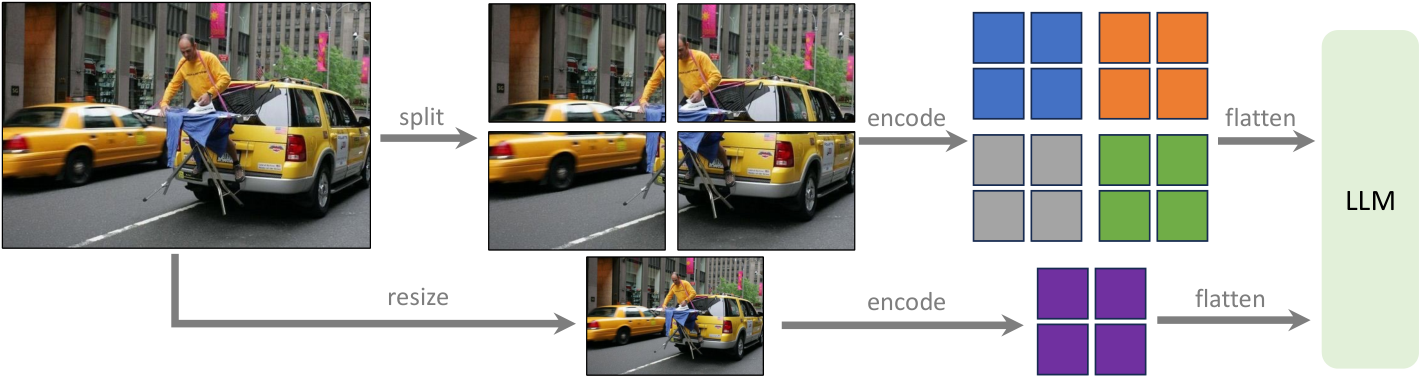
\includegraphics[width=\linewidth,height=0.28\textheight,keepaspectratio]{images/vision-language-models/llava15_fig2_hd_tiling.png}\\[0.2em]
  {\scriptsize LLaVA-1.5-HD. Liu et al., \href{https://arxiv.org/abs/2310.03744v2}{arXiv:2310.03744v2}, Figure~2, Sec.~3.4, App.~A.1; the LLaVA-NeXT post uses the same diagram.\par}
  \vspace{0.3em}
  \begin{columns}[T,onlytextwidth]
    \column{0.50\textwidth}
      \begin{itemize}\footnotesize\itemsep0.3em
        \item \textbf{LLaVA-1.5-HD:} open CLIP encoders then stopped at 336 px, so HD tiles the padded image at its encoder's native 224 px (up to six tiles, e.g.\ $2\times3$ or $1\times6$) and encodes each tile alone. A 224 px whole-image view is added, and a row-end token closes each feature row.
        \item \textbf{LLaVA-NeXT AnyRes} (Jan.\ 2024): 336 px tiles; the post lists $2\times2$, $1\times\{2,3,4\}$ and $\{2,3,4\}\times1$ grids, up to $1344\times336$ (released configs stop at $1008\times336$), ``4x more pixels'' than LLaVA-1.5.
      \end{itemize}
    \column{0.48\textwidth}
      \begin{itemize}\footnotesize\itemsep0.3em
        \item \textbf{Tokens:} a $2\times2$ grid of 336 px tiles plus a 336 px global view gives $4\times576 + 576 = 2{,}880$ visual tokens before row-end tokens: $5\times$ LLaVA-1.5 and over $11\times$ LLaVA.
        \item \textbf{Context:} Vicuna v1.5 reads 4,096 tokens: one such image fills about 70\% of them before any text, and two do not fit.
      \end{itemize}
  \end{columns}
  \vspace{0.2em}
  {\scriptsize Source: Liu et al., ``LLaVA-NeXT: Improved reasoning, OCR, and world knowledge,'' LLaVA blog, 30 Jan.\ 2024, \href{https://llava-vl.github.io/blog/2024-01-30-llava-next/}{llava-vl.github.io/blog/2024-01-30-llava-next}. Global view: \texttt{llava/mm\_utils.py}, \href{https://github.com/haotian-liu/LLaVA}{github.com/haotian-liu/LLaVA}; context: \href{https://huggingface.co/liuhaotian/llava-v1.6-vicuna-13b/blob/main/config.json}{llava-v1.6-vicuna-13b config}.\par}
\end{frame}
